\documentclass[twoside,10pt,a4paper]{article}
\usepackage[utf8]{inputenc}
\usepackage[english]{babel}
\usepackage{amsmath}
\usepackage{amsfonts}
\usepackage{amssymb}
\usepackage{graphicx}

\usepackage[left=2cm,right=2cm,top=2cm,bottom=3cm]{geometry}
\usepackage{fancyvrb}
\usepackage{listings}
\usepackage{xparse}
\usepackage{tikz} % ajout de dessins LaTeX
\usepackage{graphicx}
\usepackage{float}  % alignement des figures
\usepackage{fancyhdr}
\usepackage{enumitem}
\usepackage{verbatim}
\usepackage{xcolor}

\usepackage{caption}
\usepackage{subcaption}

\pagestyle{fancy} %fancyhdr
	\fancyhf{} %fancyhdr
	\renewcommand{\sectionmark}[1]{\markboth{#1}{}}
	\fancyhead[R]{NLDCI Set 3 Solutions} %INSERT TITLE HERE FOR fancyhdr
	\fancyhead[L]{\nouppercase{\leftmark}} %fancyhdr
	\cfoot{\thepage} %fancyhdr
	\setlength{\headheight}{35pt}
	\setlength{\parindent}{0pt}

\begin{titlepage}
\title{\huge \textbf{Nonlinear Dynamics \& Chaos I \\ \Large Exercice Set 3 Solutions}}	%TITLE
\author{ }		%AUTHOR
\date{ }	%DATE

\end{titlepage}

	\definecolor{MyBlue}{HTML}{4A90E2}
	\definecolor{MyRed}{HTML}{D0021B}


\begin{document}

\maketitle

\section*{Question 1}
Consider a ball of mass $m$ that slides on a rotating hoop (see Fig. \ref{Q01D01}).

\begin{figure}[H]
	\centering
	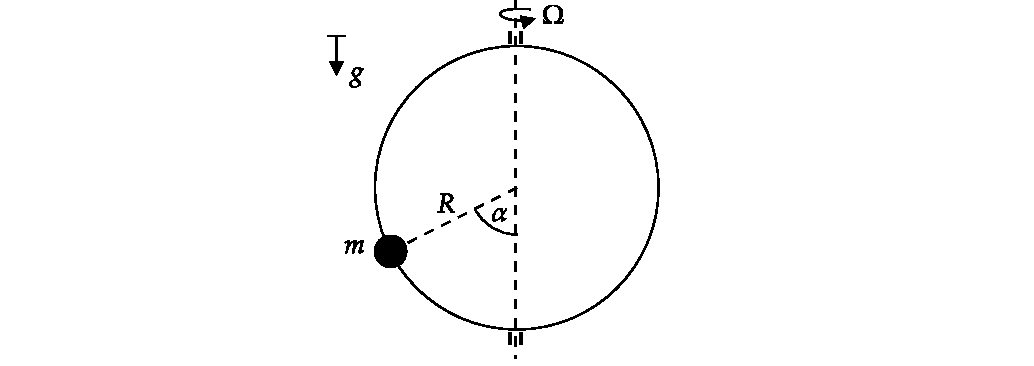
\includegraphics[scale=0.9]{Graphics/Q01D01.pdf}
	\caption{Mass on a hoop}
	\label{Q01D01}
\end{figure}
The angular velocity of the hoop is $\Omega$, the viscous friction coefficient between the hoop and the ball is $b$, and the constant of gravity in $g$. The equation of motion for the sliding ball is given by
\begin{equation*}
	mR^2 \ddot{\alpha} + bR^2 \dot{\alpha} + mR^2(g/R - \Omega^2 \cos(\alpha)) \sin(\alpha) = 0.
\end{equation*}
\begin{enumerate}[label=(\alph*)]
	\item Plot the location of equilibria of the ball as a function of the non-dimensionalized rotation parameter $\nu = R\Omega^2 /g$.
	\item Using linearization, determine the stability type of the different equilibrium branches on the plot. Identify the critical angular velocity at which a bifurcation of equilibria occurs.
\end{enumerate}

\section*{Solution 1}
\begin{enumerate}[label=(\alph*)]
\item The equation of motion for the sliding ball is given by
\begin{equation*}
	mR^2 \ddot{\alpha} + bR^2 \dot{\alpha} + mR^2(g/R - \Omega^2 \cos (\alpha))\sin (\alpha) = 0
\end{equation*}
Where we'll define $\nu = R\Omega^2 /g$

We can define $x_1 = \alpha, \,\, x_2 = \dot{\alpha}$ in order to write the ODE as $\dot{x} = f(x)$ where
\begin{equation*}
	x = \begin{pmatrix}
		x_1 \\
		x_2
	\end{pmatrix}
	\qquad \text{and} \qquad f(x) = \begin{pmatrix}
		x_2 \\
		-\displaystyle \frac{g}{R}[1-\nu \cos (x_1)]\sin (x_1) - \frac{b}{m} x_2
	\end{pmatrix}
\end{equation*}
In other words
\begin{equation*}
	\begin{bmatrix}
		\dot{x_1} \\
		\dot{x_2}
	\end{bmatrix} = \begin{bmatrix}
		x_2 \\
		-\displaystyle \frac{g}{R}[1-\nu \cos (x_1)]\sin (x_1) - \frac{b}{m} x_2
	\end{bmatrix}
\end{equation*}
Fixed points are found when $f(x)=0$. This implies that $ x_2 =0$ and $[1-\nu \cos (x_1)]\sin (x_1)=0$

\subsubsection*{Case 1: $\nu <1$:}
Only two fixed points exist: $(0,0)$ and $(\pi,0)$ [Note: the fixed point $(-\pi,0)$ is physically identical to the fixed point $(\pi,0)$. Therefore, we only discuss $(\pi,0)$]

\subsubsection*{Case 2: $\nu >1$:}
Two additional fixed points emerge that correspond to the solutions of $\cos(x_1) = \frac{1}{\nu}$.

Let $\alpha_0 \in (0,\pi)$ be the positive solution: $\cos(\alpha_0) = \frac{1}{\nu}$. Then the fixed points in this case are: 

$(0,0),(\pi,0),(\alpha_0,0)$ and $(-\alpha_0,0)$

\begin{figure}[H]
	\centering
	
\includegraphics[scale=0.9]{Graphics/S01D01.pdf}
\end{figure}
The blue curves mark the location of the fixed points.


\item First we compute $\nabla f(x_1, x_2)$:
\begin{equation*}
	\nabla f(x_1, x_2) = \begin{pmatrix}
		0 & 1 \\
		\displaystyle \frac{g}{R}[2\nu \cos^2(x_1) - \cos(x_1) - \nu] & \displaystyle -\frac{b}{m}
	\end{pmatrix}
\end{equation*}
who's eigenvalues are given by
\begin{equation*}
	\lambda_\pm = -\frac{b}{2m} \pm \sqrt{\left(\frac{b}{2m}\right)^2 + \frac{g}{R}[2\nu \cos^2(x_1) - \cos(x_1) - \nu]}
\end{equation*}
Now we investigate the linear stability of each fixed point:
\subsubsection*{Fixed point $(0,0)$:}
\begin{equation*}
	\lambda_\pm = -\frac{b}{2m} \pm \sqrt{\left(\frac{b}{2m}\right)^2 + \frac{g}{R}(\nu -1)}
\end{equation*}
\begin{itemize}
	\item $\nu < 1 \Longrightarrow$ Re$(\lambda_+)<0$ and Re$(\lambda_-)<0$. Therefore $(0,0)$ is asymptotically stable.
	
	\item $\nu > 1 \Longrightarrow$ Re$(\lambda_+)>0$ and Re$(\lambda_-)<0$. Therefore $(0,0)$ is unstable.
\end{itemize}

\subsubsection*{Fixed points $(\pm \pi,0)$:}
\begin{equation*}
	\lambda_\pm = -\frac{b}{2m} \pm \sqrt{\left(\frac{b}{2m}\right)^2 + \frac{g}{R}(\nu + 1)}
\end{equation*}
For any $\nu \geq 0$, Re$(\lambda_+)>0 \Longrightarrow (\pm \pi,0)$ is unstable for any $\nu \geq 0$.


\subsubsection*{Fixed points $(\pm \alpha_0,0)$}
Remember that these fixed points only exist when $\nu > 1$. Also $\cos(\pm \alpha_0) = \frac{1}{\nu}$
\begin{equation*}
	\lambda_\pm = -\frac{b}{2m} \pm \sqrt{\left(\frac{b}{2m}\right)^2 + \frac{g}{R}\left( \frac{1-\nu^2}{\nu} \right)}
\end{equation*}
For any $\nu > 1$, Re$(\lambda_+)<0$ and Re$(\lambda_-)<0$. Therefore the fixed points $(\pm \alpha_0,0)$ are asymptotically stable. 

\begin{figure}[H]
	\centering
	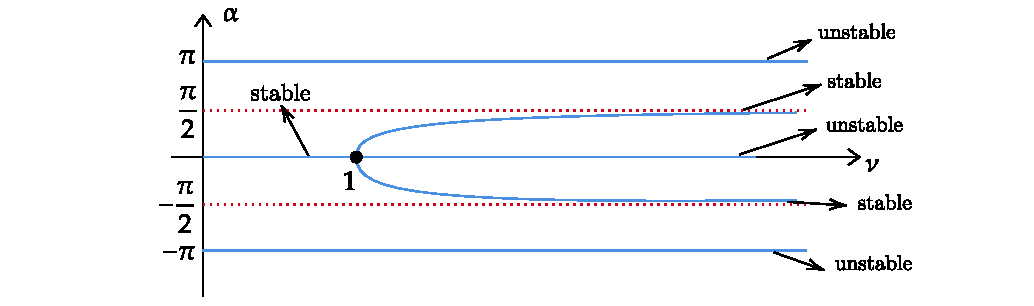
\includegraphics[scale=0.9]{Graphics/S01D02.pdf}
\end{figure}

The bifurcation of equilibria occurs at $\nu = 1 \Longrightarrow \Omega^2 = \frac{g}{R} \Longrightarrow \Omega = \pm \sqrt{\frac{g}{R}}$

\end{enumerate}

\newpage

\section*{Question 2}
Consider a discrete dynamical system given by the iterated mapping
\begin{equation*}
	x_{k+1} = f(x_k), \qquad f: \mathbb{R}^n \rightarrow \mathbb{R}^n, \qquad x_k \in \mathbb{R}^n.
\end{equation*}
Assume that $x = p$ is a fixed point for the mapping, i.e., $p = f(p)$.

\begin{enumerate}[label=(\alph*)]
	\item Derive a linearized mapping of the form
	\begin{equation}\label{Q02E01}
		y_{k+1} = Ay_k
	\end{equation}
	to describe the discrete dynamics in the vicinity of the fixed point.
	\item Assume that $A$ has eigenvalues $\lambda_1, \ldots, \lambda_n \in \mathbb{C}$ with corresponding $n$ linearly independent eigenvectors $s_1, \ldots, s_n \in \mathbb{C}^n$. Show that the general solution of (\ref{Q02E01}) is of the form
	\begin{equation}\label{Q02E02}
		y_k = c_1 \varphi_1(k) + \cdots + c_n \varphi_n(k), \qquad \varphi_i(k) = \lambda_i^ks_i.
	\end{equation}
	\item Formulate a definition of stability, asymptotic stability, and instability for the $y=0$ fixed point of (\ref{Q02E01}).
	\item Using (\ref{Q02E02}), find a sufficient and necessary condition for the asymptotic stability you have defined in (c).
\end{enumerate}

\section*{Solution 2}
\begin{enumerate}[label=(\alph*)]
\item Let $x_k$ be near the fixed point $P$ and define $y_k = x_k - P$. Then
\begin{align*}
	x_{k+1} = f(x_k) = f(P + y_k) &= f(P) + Df(P)y_k + \mathcal{O}(||y_k||^2) \\
	&= P + Df(P)y_k + \mathcal{O}(||y_k||^2)
\end{align*}
\begin{equation*}
	\Longrightarrow y_{k+1} = x_{k+1} - P = Df(P)y_k + \mathcal{O}(||y_k||^2)
\end{equation*}
Now for $||y_k||$ small enough the linear approximation of the map $x_{k+1} = f(x_k)$ is $y_{k+1} = Ay_k$ with $A = Df(P)$.


\item Take any $y_0 \in \mathbb{R}^n$. Since $s_1,\ldots ,s_n \in \mathbb{C}^n$ are linearly independent there are constants $c_1,\ldots ,c_n \in \mathbb{C}$ such that $y_0 = c_1s_1+\ldots+c_ns_n$.

Now define
\begin{align*}
	y_1 = Ay_0 &= c_1As_1 + \cdots + c_nAs_n \\
	&= c_1\lambda s_1 + \cdots + c_n\lambda s_n \\
	&= c_1\varphi_1(1) + \cdots + c_n \varphi_n(1)
\end{align*}
Similarly, for any $k \geq 1$,
\begin{align}
	y_k = Ay_{k-1} &= c_1 \lambda_1^{k-1}As_1 + \cdots + c_n \lambda_n^{k-1}As_n \nonumber \\
	&= c_1\varphi_1(k) + \cdots + c_n \varphi_n(k)
\end{align}
It's easy to check that $y_{k+1} = Ay_k$ for any $k \geq 0$. Since $y_0 \in \mathbb{R}^n$ was arbitrary, $c_1\varphi_1(k)+c_2\varphi_2(k) + \cdots + c_n\varphi_n(k)$ is a general solution of $y_{k+1} = Ay_k$.


\item \subsubsection*{Definition of stability:}
\begin{equation*}
	\,\forall \varepsilon > 0, \exists \delta(\varepsilon)>0 \text{ such that } \,\forall y_0\in\mathbb{R}^n \text{ with } ||y_0|| \leq \delta \text{ we have } ||y_k|| \leq \varepsilon \text{ for any } k \geq 0
\end{equation*}

\subsubsection*{Definition of asymptotic stability:}
$y = 0$ is asymptotically stable if and only if:
\begin{itemize}
	\item $y=0$ is stable
	\item $\exists \delta > 0$ such that $\,\forall y_0 \in \mathbb{R}^n$ with $||y_0||<\delta$ we have $\displaystyle \lim_{k \rightarrow \infty} ||y_k|| = 0$	
\end{itemize}

\subsubsection*{Definition of instability:}
$y=0$ is unstable if it's \underline{not} stable !


\item We claim that the necessary and sufficient condition for asymptotic stability of the origin is $|\lambda_i|<1$ for $i=1,2,\ldots , n$

\underline{Sufficient}: From (c) any solution of $y_{k+1} = Ay_k$ can be written as:
\begin{equation*}
	y_{k+1} = \sum_{i=1}^n c_i \lambda_i^k s_i
\end{equation*}
Without loss of generality, we assume that the eigenvectors $s_i$ are normalized, i.e., $||s_i|| = 1 \,\forall i\in\{1,2,\ldots,n\}$. Then
\begin{equation*}
	||y_{k+1}|| \leq \sum_{i=1}^n |c_i||\lambda_i|^k ||s_i|| = \sum_{i=1}^n |c_i||\lambda_i|^k
\end{equation*}
But since $|\lambda_i|<1$, we have $\displaystyle \lim_{k \rightarrow \infty} |\lambda_i|^k = 0$. Which implies
\begin{equation*}
	\lim_{k \rightarrow \infty} \sum_{i=1}^n |c_i||\lambda_i|^k = 0
\end{equation*}
Hence, 
\begin{equation}\label{E0401}
	\lim_{k \rightarrow \infty} ||y_{k+1}||=0
\end{equation}
Also note that since $|\lambda_i|<1 \,\forall i\in \{1,\ldots,n\}$, the matrix norm $||A||<1$.

Hence $||y_{k+1}|| = ||Ay_k|| < ||y_k||. \Longrightarrow y=0$ is also stable. This together with (\ref{E0401}) implies asymptotic stability of the fixed point $y=0$.

\underline{Necessity}: Assume there is $i_0\in\{1,2,\ldots, n\}$ such that $|\lambda_{i_0}| \geq 1$.

It is enough to show that $\exists y_0 {\color{red}\in\mathbb{R}^n}$ such that $\lim_{k \rightarrow \infty} ||A^ky_0|| \neq 0$

[This is due to the fact that $y_k = A^ky_0$ and that one can rescale $y_0$ as $ry_0$ for $0<r \ll 1$ small enough such that $||ry_0||<\delta, \,\forall \delta > 0$]

To show that such $y_0 \in \mathbb{R}^n$ exists, note that $||A^ks_{i_0}|| = ||\lambda_{i_0}^ks_{i_0}|| = |\lambda_{i_0}|^k \geq 1 \,\forall k \geq 0$.
\begin{center}
	\color{red} This is, however, not enough since $s_{i_0}\in\mathbb{C}^n$ while we need a vector in $\mathbb{R}^n$.
\end{center}
To complete the proof, note that $s_{i_0}=\xi + i\eta$ with $\xi, \eta \in \mathbb{R}^n$.
\begin{equation*}
	\Longrightarrow 1 \leq ||A^ks_{i_0}||^2 = ||A^k\xi + i A^k\eta ||^2 = ||A^k\xi||^2 + ||A^k\eta||^2
\end{equation*}
Therefore, either $||A^k\xi|| \geq \frac{1}{\sqrt{2}}$ or $||A^k\eta|| \geq \frac{1}{\sqrt{2}}$.

Without loss of generality assume $||A^k\xi|| \geq \frac{1}{\sqrt{2}}$. Now let $y_0 = \xi$ to get
\begin{equation*}
	\underbrace{||y_k|| = ||A^ky_0|| \geq \frac{1}{\sqrt{2}}}_{\text{true for every }k\geq 0} \Longrightarrow \lim_{k \rightarrow \infty} ||y_k|| \neq 0
\end{equation*}

\end{enumerate}

\newpage

\section*{Question 3}
The first three modes of a convecing fluid motion in a two-dimensional layer heated from below are described by the famous \textit{Lorenz equations}
\begin{align*}
	\dot{x} &= a(y - x), \\
	\dot{y} &= bx - y - xz, \\
	\dot{z} &= xy - cz.
\end{align*}
Here $a>0$ denotes the Prandtl number, $b>0$ is the Rayleigh number, and $c>0$ is the aspect ratio. Lorenz's original assumption is that $a > 1 + c$.

The above equations describe the evolution of the amplitudes of one velocity mode and two temperature modes. As a paradigm of chaotic dynamics, this system has inspired much of the development of the modern geometric theory of dynamical systems.

\begin{enumerate}[label=(\alph*)]
	\item Complicated dynamics arise when all possible equilibria of the system become unstable, and hence solutions cannot settle down to any simple steady state. Show that this is the case when
	\begin{equation*}
		b > \frac{a(3 + a + c)}{a - c - 1}
	\end{equation*}
	\textit{Note}: Note: A negative sign for one of the Routh-Hurwitz determinants actually implies instability, not just the lack of asymptotic stability.
	\item Solve the Lorenz equations numerically for $a=10$, $b=28$, and $c=8/3$, choosing an initial condition close to $x=y=z=0$. Plot the trajectory in three dimensions to show that it converges to a complicated surface, a \textit{chaotic attractor}.
\end{enumerate}

\section*{Solution 3}
\begin{enumerate}[label=(\alph*)]
\item By setting $f(x)=0$, we obtain three fixed points for $\dot{x} = f(x)$. This can be seen by noting that the first equation $a(y_0 - x_0)=0$ implies $x_0 = y_0$. From the second equation, we get
\begin{align*}
        &bx_0 - y_0 -x_0 z_0 = 0 \\
	&z_0 = b-1.
\end{align*}

Then the third equation reduces to
\begin{align*}
        &x_0y_0 - cz_0 = 0\\
        	&x_0=y_0 = \pm \sqrt{c(b-1)}.
\end{align*}
The resulting three fixed points are
\begin{align*}
	P_1 &: x_0 = y_0 = z_0 = 0\\
	P_2 &: x_0 = y_0 = \sqrt{c(b-1)} \;, z_0 = b-1 \\
	P_3 &: x_0 = y_0 = -\sqrt{c(b-1)} \;, z_0 = b-1.
\end{align*}
For the system to have these three fixed points we must have $\boxed{b>1}$. If $0<b\leq1$, the only fixed point is $P_1$.

Let $A$ denote $Df(x_0,y_0,z_0)$. Then:
\begin{equation*}
	A = \begin{pmatrix}
		-a & a & 0 \\
		b-z_0 & -1 & -x_0 \\
		y_0 & x_0 & -c
	\end{pmatrix}
\end{equation*}

The eigenvalues $\lambda$ of $A$ are defined as the roots of the characteristic polynomial
$$
\det |A - \lambda I |=0.
$$
For the matrix $A$ this takes the form
\begin{equation*}
	A = \begin{vmatrix}
		-a-\lambda & a & 0 \\
		b-z_0 & -1-\lambda & -x_0 \\
		y_0 & x_0 & -c-\lambda
	\end{vmatrix} = 0.
\end{equation*}
We may expand this determinant according to the first row as

\begin{align*}
&(-a-\lambda)\begin{vmatrix}-1-\lambda & -x_0 \\ x_0 & -c-\lambda \end{vmatrix} - a \begin{vmatrix} b-z_0 & -x_0 \\ y_0 & -c-\lambda \end{vmatrix} =0 \\
&-(a+\lambda)\left[ (1+\lambda) (c+\lambda) + x_0^2 \right] -a(b-z_0)(-c-\lambda) -ax_0y_0= 0
\end{align*}
After collecting the coefficients of the different powers of $\lambda$, the characteristic equation of $A$ is:
\begin{equation*}
	\lambda^3 + (a+c+1)\lambda^2 + [ac + a + c + x_0^2 + a(z_0 - b)]\lambda + ac(z_0 - b + 1) + x_0^2a + ax_0y_0 = 0
\end{equation*}


\subsubsection*{Stability of $P_1$:}
\begin{equation*}
	\lambda_3 + (a + c + 1)\lambda^2 + (ac + a + c -ab)\lambda - ac(b-1) = 0
\end{equation*}
A necessary condition for all roots of the above polynomial to be negative is that all its coefficients have the same sign. But here $-ac(b-1)<0$ while $\lambda^3$ has a positive coefficient (i.e. $+1$). $\Longrightarrow A$ has a positive eigenvalue.

$\Longrightarrow P_1$ is unstable.

\subsubsection*{Stability of $P_2, P_3$:}
Note that in the characteristic equation, we only have products of $x_0$ and $y_0$, i. e. $x_0^2$ and $x_0y_0$. This means that the equation is invariant to changing the sign of $x_0$ and $y_0$ and we get the same eigenvalues at $P_2$ and at $P_3$. 

The Routh-Hurwitz determinants are:
\begin{align*}
	d_1 &= 2ac(b - 1) > 0 \\
	d_2 &= (a + b)c > 0 \\
	d_3 &= \begin{vmatrix}
		(a + b)c & 2ac(b - 1) \\
		1 & a + c + 1
	\end{vmatrix} = (a + b)(a + c + 1)c - 2ac(b - 1)
\end{align*}
For $P_2$ and $P_3$ to be unstable, we must have $d_3 < 0$
\begin{equation*}
	d_3 < 0 \Longleftrightarrow b > \frac{a(3 + a + c)}{a - (c + 1)} \underbrace{>}_{\text{follows from }a>c+1} 1
\end{equation*}

\item
\begin{Verbatim}[numbers = left]
	%% Initiate Script
	close all
	clear all
	clc
	
	%% Params & Initial Condition
	
	a = 10;
	b = 28;
	c = 8/3;
	
	x0 = [0.101; 0.1; 0.1];
	
	%% Function & Simulation
	
	f = @(t,x) [a * (x(2) - x(1));
	            b * x(1) - x(2) - x(1) * x(3);
	            x(1) * x(2) - c * x(3)];
	        
	[t ,x] = ode45(f, [0, 1000], x0);
	
	%% Plot
	
	figure(1)
	hold on
	plot3(x(:,1), x(:,2),x(:,3))
\end{Verbatim}

\newpage

\begin{figure}[H]
	\centering
	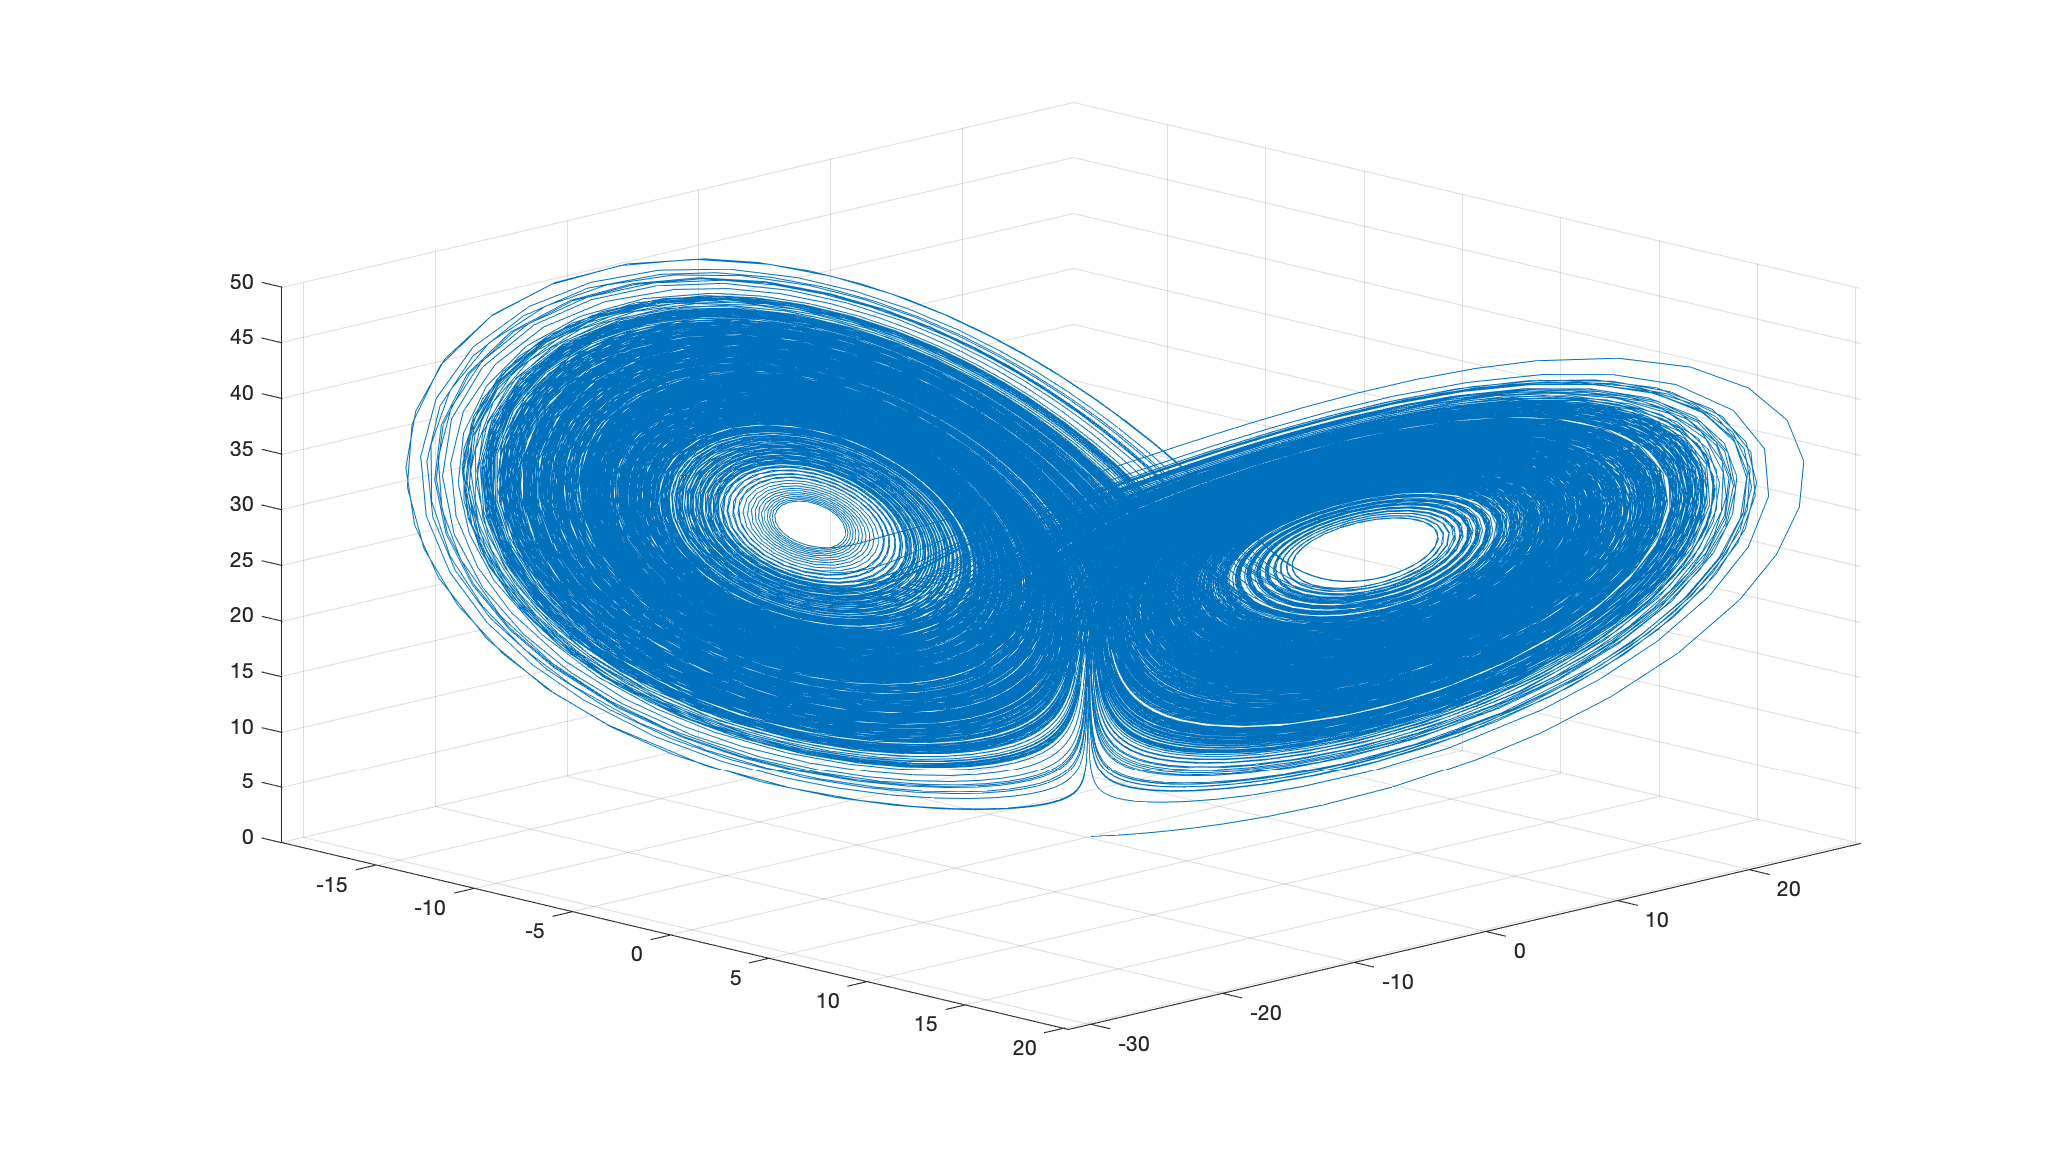
\includegraphics[scale=0.48]{Graphics/S03D01.eps}
	\caption{Simulation of the Lorenz equations.}
\end{figure}

\end{enumerate}

\newpage

\section*{Question 4}
Recall from Question 1 that a ball of mass $m$ sliding on a hoop rotating with angular velocity $\Omega$ satisfies the differential equation
\begin{equation}\label{Q04E01}
	mR^2 \ddot{\alpha} + mR^2(g/R - \Omega^2 \cos(\alpha)) \sin(\alpha) = 0
\end{equation}
if there is no friction between the hoop and the mass. Assume that the parameter values are such that the lower equilibrium position of the ball is stable in linear approximation.

\begin{enumerate}[label=(\alph*)]
	\item Show that in this case, the equilibrium is also nonlinearly stable. 
	
	\textit{Hint}: Note that system (\ref{Q04E01}) is not conservative: an external torque is required to maintain the constant rotation of the hoop. As a result, the total mechanical energy of the system is not expected to work as a Lyapunov function. To find another candidate for a Lyapunov function, find a quantity that \textit{is} conserved along trajectories. Such a quantity can be found by multiplying equation (\ref{Q04E01}) by $\dot{\alpha}$ and integrating in time.
	\item Prove that the equilibrium \textit{cannot} be asymptotically stable for the nonlinear system.
	
	\textit{Hint}: use the Lyapunov function you have found in (a).
\end{enumerate}

\section*{Solution 4}
\begin{equation*}
	mR^2\ddot{\alpha} + mR^2[g/R - \Omega^2 \cos(\alpha)]\sin(\alpha) = 0
\end{equation*}
From the previous assignment, we know that the lower equilibrium is \underline{unstable} when $\Omega^2 > g/R$. Hence, in the following we assume
\begin{equation}\label{S03E021}
	\Omega^2 < \frac{g}{R}
\end{equation}

\begin{enumerate}[label=(\alph*)]
\item Multiplying the equation of motion by $\dot{\alpha}$, we find that
\begin{equation}\label{S03E022}
	\frac{d}{dt} \left( \frac{1}{2}\dot{\alpha}^2 - \frac{g}{R}\cos(\alpha) + \frac{1}{4}\Omega^2 \cos(2\alpha) \right) = 0
\end{equation}

Let $x_1 := \alpha, x_2 := \dot{\alpha}$. Equation (\ref{S03E022}) implies that the function
\begin{equation*}
	V(x_1,x_2) = \frac{1}{2}x_2^2 + \frac{g}{R}(1 - \cos(x_1)) + \frac{\Omega^2}{4}(\cos(2x_1) - 1)
\end{equation*}
is constant along trajectories, i.e. $\frac{d}{dt}V(x_1(t),x_2(t))=0$.

Moreover, $V(0,0)=0$. On the other hand:
\begin{equation*}
	\nabla V(0,0) = \begin{pmatrix}
	0 \\0
	\end{pmatrix}
	\text{ and } \nabla^2V(0,0) = \begin{pmatrix}
		\displaystyle \frac{g}{R} - \Omega^2 & 0 \\
		0 & 1
	\end{pmatrix}
\end{equation*}
It follows from (\ref{S03E021}) that $\nabla^2V(0,0)$ is positive definite.

$\Longrightarrow$ By Lyapunov's direct method, the lower equilibrium is stable.


\item The fixed point $(0,0)$ cannot be asymptotically stable since the trajectories of the system coincide with level curves of $V(x_1,x_2)$. since $\frac{dV}{dt}=0$ along trajectories. But the above analysis shows that around $(0,0)$ the level curves of $V$ are closed curves:

\begin{figure}[H]
	\centering
	
\includegraphics[scale=0.9]{Graphics/S04D01.pdf}
\end{figure}

\end{enumerate}

\newpage

\section*{Question 5}
Consider the damped pendulum equation
\begin{equation}\label{Q05E01}
	\ddot{x} + c\dot{x} + \sin(x) = 0.
\end{equation}

\begin{enumerate}[label=(\alph*)]
	\item Using the energy of the pendulum as a Lyapunov function, can we conclude the nonlinear asymptotic stability of the $x=0$ equilibrium ? Give detailed reasoning why.
	\item A theorem due to Krasovski states the following: Assume that $x=0$ is a fixed point for the $n$-dimensional dynamical system $\dot{x}=f(x)$. Assume that there exists a smooth scalar function $V(x)$ such that
	\begin{enumerate}[label=(\roman*)]
		\item $V(x)$ is positive definite on an open neighborhood $U$ of $x=0$
		\item $\dot{V}$ is negative semi-definite on the same neighborhood
		\item the only trajectory lying \textit{completely} in the set $S= \{ x\in U \, : \, \dot{V}=0 \}$ is the fixed point $x=0$. Then $x=0$ is asymptotically stable.
	\end{enumerate}
	Use Krasovski's theorem to conclude the asymptotic stability of the origin for (\ref{Q05E01}).
\end{enumerate}

\section*{Solution 5}
\begin{enumerate}[label=(\alph*)]
\item 
\begin{equation*}
	E(x,\dot{x}) = \frac{1}{2}\dot{x}^2 + (1 - \cos(x))
\end{equation*}
\begin{align*}
	y &= (y_1,y_2) := (x, \dot{x}) \\
	y &= f(y) = \begin{bmatrix}
		y_2 \\
		-cy_2 - \sin(y_1)
	\end{bmatrix} \Longrightarrow
	E(y) = \frac{1}{2}y_2^2 + (1 - \cos(y_1))
\end{align*}

\begin{enumerate}[label=(\roman*)]
\item 
\begin{equation*}
	E(0) = 0, DE(0) = 0, D^2E(0) = \begin{bmatrix}
	1 & 0 \\ 0 & 1
	\end{bmatrix}
\end{equation*}
$\Longrightarrow$ Hessian is positive definite.

$\Longrightarrow E$ is positive-definite near the origin

\item 
\begin{align*}
	\dot{E}(y) &= \langle DE(y),f(y) \rangle = (\sin(y_1),y_2) \cdot (y_2, -cy_2 - \sin(y_1)) \\
	&= \sin(y_1)y_2 - cy_2^2 -\sin(y_1)y_2 \\
	&= -cy_2^2 \leq 0
\end{align*}
$E$ is positive definite around the origin and $\dot{E}$ is negative semi-definite.

Indeed, we cannot find an open set $U$ around the origin where
\begin{equation*}
	\dot{E}(y)<0 \;\; \forall y \in U\backslash \{0\} \;\; [\dot{E}(y)=0 \text{ for any } y = (y_1,0) \text{ with } y_1 \neq 0]
\end{equation*}
Thus, theorem 2 is not applicable to conclude nonlinear asymptotic stability of the origin.

\end{enumerate}


\item We use Krasovski's theorem with $V = E, U \subset (-\pi, \pi) \times \mathbb{R}$ open set around the origin in $S' \times \mathbb{R}$ such that the statements (i) \& (ii) in the hypothesis of Krasovski are satisfied as shown above in part a).

\begin{equation}
	S = \{ y \in U \vert \dot{E}(y)=0 \} \subset \underbrace{\{ (y_1, 0) \;\vert\; y_1 \in (-\pi,\pi) \}}_{\tilde{S}}
\end{equation}
Indeed, the only trajectory of the system completely contained in the set $\tilde{S}$ on the $y_1$-axis is the origin (cf. phase portrait). $\Longrightarrow S$ contains only the fixed point as a trajectory of the system.

Hence, the hypothesis of Krasovski's theorem is satisfied and the origin is asymptotically stable for the nonlinear damped pendulum.

\end{enumerate}

\newpage

\section*{Question 6}
Consider an $n$-degree-of-freedom holonomic mechanical system (i.e. one that has only position-dependent constraints) with generalized coordinates $q\in \mathbb{R}^n$ and generalized velocities $\dot{q}\in \mathbb{R}^n$. The total energy of the system is of the form
\begin{equation*}
	E(q, \dot{q}) = \frac{1}{2} \dot{q}^T M(q)\dot{q} + V(q),
\end{equation*}
where $M \in \mathbb{R}^{n \times n}$ is the mass matrix (symmetric ans positive definite), and $V(q)$ is the potential energy. In the absence of external forces, the associated Lagrangian equations of motion are
\begin{equation*}
	\frac{d}{dt} \frac{\partial L}{\partial \dot{q}} - \frac{\partial L}{\partial q} = 0,
\end{equation*}
where $L(q, \dot{q}) = \frac{1}{2}\dot{q}^T M(q)\dot{q} + V(q)$ is the Lagrangian of the mechanical system.

Show that if $V(q)$ admits a strict local minimum at a point $q_0$, then $q_0$ is a (nonlinearly) stable equilibrium for the mechanical system. (This result is also known as \textit{Dirichlet's Theorem} in classical mechanics).

\section*{Solution 6}
First construct the function:
\begin{align*}
	\bar{E}(q, \dot{q}) &= E(q, \dot{q}) - V(q_0) \\
	&= \frac{1}{2}\dot{q}^\text{T}M\dot{q} + V(q) - V(q_0)
\end{align*}
Now, at $(q,\dot{q})=(q_0,0)$ we have $\bar{E}(q_0,0)=0$

Note that $M(q)$ is positive definite for all $q$ and $V(q) - V(q_0)$ is positive around $q=q_0$. (Since $V$ has a local minimum at $q_0$)

$\Longrightarrow \bar{E}(q,\dot{q})$ is positive definite around $(q_0,0)$.

But $\displaystyle \frac{d\bar{E}}{dt} = \frac{dE}{dt}$ since $V(q_0)$ is a constant.

We show that $\displaystyle \frac{dE}{dt}=0$.

First note that, in general, the Lagrangian equation of motion is a system of $n$ coupled equations with each equation given by:
\begin{equation*}
	\frac{d}{dt} \left[ \frac{\partial L}{\partial \dot{q}_k} \right] - \frac{\partial L}{\partial q_k} =0 \qquad k = 1,2,\ldots,n
\end{equation*}
Multiply each equation by $\dot{q}_k$ and sum over $k$ to get:

{\color{red} (We'll use Einstein's notation: sum over repeated indices)}

\begin{equation}\label{S03E041}
	\dot{q}_k \left[ \frac{d}{dt}\left( \frac{\partial L}{\partial \dot{q}_k} \right) - \frac{\partial L}{\partial q_k} \right] =0
\end{equation}
Since $\displaystyle L = \frac{1}{2}M_{ij}\dot{q}_i \dot{q}_j - V$ we have:

\begin{equation}\label{S03E042}
	\begin{aligned}
		\frac{\partial L}{\partial \dot{q}_k} &= M_{ik}\dot{q}_i \quad , \quad \frac{\partial L}{\partial q_k} = \frac{1}{2} \frac{\partial M_{ij}}{\partial q_k}\dot{q}_i\dot{q}_j - \frac{\partial V}{\partial q_k} \\
		\frac{d}{dt} \frac{\partial L}{\partial \dot{q}_k} &= M_{ik}\ddot{q}_i + \frac{\partial M_{ik}}{\partial q_j}\dot{q}_j\dot{q}_i
	\end{aligned}
\end{equation}
Substituting (\ref{S03E042}) into (\ref{S03E041}), we get
\begin{equation*}
	M_{ik} \ddot{q}_i\dot{q}_k + \frac{\partial M_{ik}}{\partial q_j}\dot{q}_j\dot{q}_i\dot{q}_k - \frac{1}{2}\frac{\partial M_{ij}}{\partial q_k}\dot{q}_i\dot{q}_j\dot{q}_k + \frac{\partial V}{\partial q_k}\dot{q}_k = 0
\end{equation*}
Since there is a sum over repeated indices we have:
\begin{align*}
	M_{ik}\ddot{q}_i\dot{q}_k &\equiv M_{ij}\ddot{q}_i\dot{q}_j & \frac{\partial M_{ik}}{\partial q_j}\dot{q}_j\dot{q}_i\dot{q}_k &\equiv \frac{\partial M_{ij}}{\partial q_k}\dot{q}_i\dot{q}_j\dot{q}_k
\end{align*}
\begin{equation}
	\Longrightarrow \underbrace{M_{ij}\ddot{q}_i\dot{q}_j + \frac{1}{2} \frac{\partial M_{ij}}{\partial q_k}\dot{q}_i\dot{q}_j\dot{q}_k + \frac{\partial V}{\partial q_k}\dot{q}_k}_{ \displaystyle =\frac{d}{dt}\left[ \frac{1}{2}M_{ij}\dot{q}_i\dot{q}_j+V(q) \right]} = 0
\end{equation}
\begin{equation*}
	\Longrightarrow \left[ \frac{1}{2}\dot{q}^\text{T}M(q)\dot{q} + V(q) \right] = 0 \Longrightarrow \frac{dE}{dt}=0 \Longrightarrow \frac{d\bar{E}}{dt}=0
\end{equation*}
Using $\bar{E}$ as the Lyapunov function, we conclude that $(q_0,0)$ is a \underline{stable} equilibrium point.


\end{document}